\chapter{Advanced Use}
\label{chap:advancedUse}

\begin{chapabstract}
In this chapter we present some slightly more complicated variations on the concepts given previously in \cref{chap:basicUse}. By the end of this chapter you should be able to do most of the things that you will ever require.
\end{chapabstract}

\lettrine[lines=2,slope=5pt,findent=4pt,nindent=0pt]{M}{any} useful time-saving commands are included. The simplest of these are a list of common abbreviations: \eg \ie \etc, \naive, \cpright, \dprime, \about; and their uppercase equivalents: \Ie \Eg \etc (see \sref{sec:abbreviations} file for full list). Also included are custom environments for \marginnote{\textsc{Example note}}{margin notes}, and named quotes:

\begin{quotetext}{Me, just now}
The meaning of a word is in its use
\end{quotetext}

Additional information can be placed in footnotes, such as this\footnote{An example footnote}, or in an endnote, like this\endnote{An example endnote}. The endnotes will appear where-ever the user includes the \verb|\theendnotes| command (usually towards the end of the chapter). Bigger chunks of information can be placed in a thesis appendex (\eg \aref{dfd}), which appears at the end of the document, or in a chapter appendix (\eg \aref{sec:exampleAppendixII}). Glossary symbols can be referred to, thus: \gls{exterm}. The name of the glossary term can also be referred to, thus: \glstext{exterm}. Once a term has been referenced it will appear in the nomenclature at the start of the document, which will automatically be linked-to. Edit \verb|_glossary/glossary.tex| to add/remove/modify entries.

% ==============================================================================================
\section{Graphics, tables and equations}

%------------------------------------------------------------------------------
\subsection{Advanced figures}
often we want to place figures side-by-side. As demonstrated in \fref{fig:exampleSideBySide}, this can be achieved using the \verb|subfloatrow| environment. If you prefer, you can replace this with similar packages such as \verb|subfig| or \verb|subfigure|. However, \verb|subfloatrow|, appears more flexible (albeit a bit more tricky to get the hang of).


\begin{figure}[H]
\ffigbox{
  \begin{subfloatrow}
  \floatsetup{ 
  	heightadjust=object,
 	 valign=b % align on bottom of image
	}
    \ffigbox[\FBwidth]{%
      	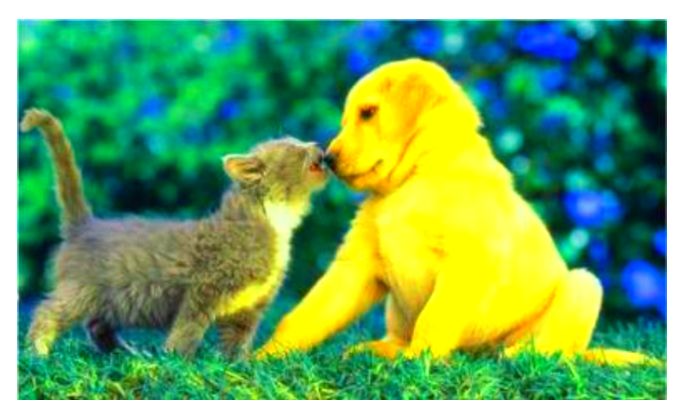
\includegraphics[scale = .25]{figs/exampleFigure}
    	}{\subcaption{} \label{fig:subFigI}}
    \ffigbox[\FBwidth]{%
      	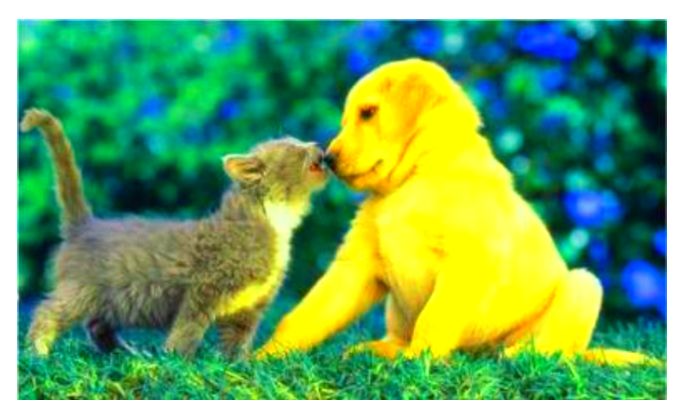
\includegraphics[scale = .35]{figs/exampleFigure}
    	}{\subcaption{} \label{fig:subFigII}}
  \end{subfloatrow}
}{
\caption[An example side-by-side figure]
{
An example side-by-side figure. Arranged using \texttt{subfloatrow}.
}
\label{fig:exampleSideBySide}
}
\end{figure}

Some users may also want to use \LaTeX's graphics engine to draw diagrams programmatically. For example, \fref{fig:exampleTikz} was generated at run-time from the commands stored in \verb|tikz_example.tex|.

\begin{figure}[H]
\centering
%\pgfmathdeclarefunction{cgauss}{2}{%
%  \pgfmathparse{0.5 * (1 - 1/30 * (7*exp(-(x^2)/2) + 16*exp(-x^2 * (2-sqrt(2))) + (7 + 1/4 * pi * x^2)*exp(-x^2) ))}% Bagby (1995)  cdf approximation
%}
\pgfmathdeclarefunction{logisticCDF}{2}{%
  \pgfmathparse{1 / (1 + exp(-(x-#1)/#2))}%
}

\begin{tikzpicture}[scale=1.1]
\begin{axis}[every axis plot post/.append style={%
  domain=-5:5,
  samples=50,
  smooth,
  },
	xmin=-2,
  	xmax=4.5,
  	ymin=0,
  	ymax=1,
	ylabel = {P(\textit{`Signal Present'})},
	xlabel = {Stimulus Strength, $x$},
	ytick={0,.25,.5,.75,1},
	%xtick={-2,0,1,2,4},
	%x tick label style={major tick length=0pt},
	%xticklabels={,0,$\Delta_{lim}$,$\Delta_{lim}$,},
	xtick={-1,0,1,2,3,4},
	xticklabels={-1,0,1,2,3,4},
  % All plots: from -2:2, 50 samples, smooth, no marks
  axis x line*=bottom, 		% no box around the plot, only x and y axis
  axis y line=left,
  enlargelimits=upper,
  legend entries={line 1, line 2, line 3},
  legend pos= south east,
  legend cell align=left,
  legend style={draw=none, font=\scriptsize} % remove border
  ] 		% extend the axes a bit to the right and top

  
  \addplot+[thick,mark=none] {logisticCDF(0,1)};
  \addplot+[thick,mark=none] {logisticCDF(-1,2)};
  \addplot+[thick,mark=none] {logisticCDF(1,1)};

  \draw[dashed, -] ({axis cs:-5,.725}) -- ({axis cs:1.96,.725});
  \draw[dashed, ->] ({axis cs:.96,.725}) -- ({axis cs:.96,0});
  \draw[dashed, ->] ({axis cs:1.96,.725}) -- ({axis cs:1.96,0});
  
  \addplot[only marks, mark=o, color=black] plot coordinates {(-1,0.5)};
  \addplot[only marks, mark=o, color=black] plot coordinates {(0,0.5)};
  \addplot[only marks, mark=o, color=black] plot coordinates {(1,0.5)};
  
\end{axis}
\end{tikzpicture}
\caption[An example tikz figure]
{
An example tikz figure. Generated at runtime from \texttt{tikz/tikz\_example.tex}.
}
\label{fig:exampleTikz}
\end{figure}

%------------------------------------------------------------------------------
\subsection{Advanced tables}

A number of table formatting packages are included (multirow, longtable, colortbl, booktabs, threeparttable, tabularx). Using these, it is possible to create quite complex tables:

\begin{table}[H]
  \centering
  \smallskip 
  \begin{threeparttable}
\begin{tabularx}{\textwidth}{>{\bfseries}l c >{\columncolor{gray}\footnotesize}*{3}{X} c *{3}{X}}
\toprule
\multirow{2}{*}{Listener} && \multicolumn{3}{c}{Analysis 1\tnote{a}} && \multicolumn{3}{c}{Analysis 2}\\[4pt]
\cmidrule(r){3-5} \cmidrule(r){7-9}
&& $F$ & $p$ & $\eta_{p}^{2}$ && $F$ & $p$ & $\eta_{p}^{2}$\\
\midrule
\rowcolor{yellow}{L1}		&& 1.2 			& .001				& 0.7	&&	0.9	& .041	& 0.3\\
L2							&& 3.3			& .001				& 0.7	&&	0.9	& .041	& 0.3\\
L3							&& 4.1			& .001				& 0.7	&&	0.9	& .041	& 0.3\\
L4							&& 5.6			& .001\tnote{b}		& 0.7	&&	0.9	& .041	& 0.3\\[12pt]
L7							&& 2.3			& .001				& 0.7	&&	0.9	& .041	& 0.3\\
L8							&& 1.7			& .001				& 0.7	&&	0.9	& \cellcolor{red}.041	& 0.3\\
L9							&& 7.9			& .001				& 0.7	&&	0.9	& .041	& 0.3\\
\bottomrule
\end{tabularx}
	\begin{tablenotes}
       \item[a] \footnotesize{See also \cite{neddis2009best}}
       \item[b] \footnotesize{Example footnote II}
	\end{tablenotes}
  \end{threeparttable}
\caption[An example complex table]
{
An example complex table. Its width adjusts to fit the page width. It includes footnotes, colour elements, and cells spanning multiple rows and/or columns.
}
\label{tab:advancedTable}
\end{table}  

Using \verb|kbordermatrix| it is also easy to generate matrices, thus:

\kbordermatrix{\text{indices}&
(1\cdot11)&(1\cdot12)&(1\cdot22)&
\vrule&
(2\cdot11)&(2\cdot12)&(2\cdot22)\\
%
(1)&\lambda(1)^2&2\lambda(1)\lambda(2)&\lambda(2)^2&\vrule&0&0&0\\
3(2)&0&0&0&\vrule&\lambda(1)^2&2\lambda(1)\lambda(2)&\lambda(2)^2\\
\hline
(111)&3&0&0&\vrule&0&0&0\\
(112)&0&2&0&\vrule&1&0&0\\
(122)&0&0&1&\vrule&0&2&0\\
(222)&0&0&0&\vrule&0&0&3}


%------------------------------------------------------------------------------
\subsection{Advanced equations}

Multi-line equations can be aligned on a common point, such as the equals sign, and text can be placed between rows. For example:
\begin{subequations}
\label{eq:pc}
\begin{align}
 E[|X|] &= \int_{x} |x| f_X(x) dx \\
 \intertext{It is thus trivial that:}
 &= \int_{|x| \ge a} \! |x| f_X(x) dx + \int_{|x| < a} \! |x| f_X(x) dx \\
 &\ge \int_{|x| \ge a} |x| f_X(x) dx \\
 \intertext{Recalling what we learnt earlier:}
 &\ge a \int_{|x| \ge a} f_X(x) dx \\
 &= a E[|X| \ge a]\\
 \intertext{Now if we add a pinch of salt:}
 \therefore \qquad E[|X| \ge a] &\le \frac{E[|X|]}{a}
\end{align}
\end{subequations} 

% not working:
%Also included is an environment, \textsc{mathlist}, which allows comma-separated lists to be broken across lines. This allows long lists to be included in the body text (inline) without risking overflows. For example the sequence: \mathlist{a,b,c,d,e,f,g,h,i,j,k,l,m,n,o,p,a,b,c,d,e,f,g,h,i,j,k,l,m,n,o,p,a,b,c,d,e,f,g,h,i,j,k,l,m,n,o,p} would normally spill into the margin, thus: $0,1,1,2,3, 5, 8, 13, 21, 34, 55, 89, 144, 233, 377, 610, 987, 1597, 2584, 4181, 6765, 10946, 17711, 28657,46368,75025,121393,196418,317811,196418,317811$\\


%------------------------------------------------------------------------------
\subsection{Code listing}

Sometimes you may want to include excerpts of code. This can be done either by typing the code directly into the file:

\begin{lstlisting}
for a=1:5
  b(a) = a*2
  c = sum(b)

  if(c > 15)
	  disp('c is big')
  end
end
\end{lstlisting}

Or by importing the code from a file
\lstinputlisting[language=matlab]{code/exampleCode.m}


% ==============================================================================================
\section{Conclusions}
In this chapter we have:
\begin{enumerate}[(1)]
\item Use various text commands
\item Add chapter appendices
\item Arrange figures
\item Customise tables
\item Align equations
\item Include code listings
\end{enumerate}


% ==============================================================================================
\theendnotes


% ==============================================================================================
\begin{chapacknowledgements}
This work was supported by the Medical Research Council, UK (Grant: U135097130).
\end{chapacknowledgements}


% ==============================================================================================
\begin{chapappendices}

%---------------------------------------------------------------
\section{An example appendix}
\label{sec:exampleAppendixI}
Here is an example chapter appendix. Further appendices can be placed at the end of the thesis, but sometimes it is nice to have appendices within the chapter itself. Each chapter appendix appears on a new page.

%---------------------------------------------------------------
\section{Another example appendix}
\label{sec:exampleAppendixII}
This is another appendix.

%---------------------------------------------------------------
\end{chapappendices}

% EOF